\chapter{Nonlocality and the boundary of reality}\label{ch:nonlocal}

\section{Bell, CHSH, Tsirelson}

Bell showed that no local hidden-variable theory can reproduce every correlation of quantum
mechanics~\cite{Bell1964}. In the CHSH form~\cite{CHSH1969}, local theories obey $|S|\le2$,
while quantum mechanics reaches the Tsirelson bound $|S|=2\sqrt2$~\cite{Tsirelson1980}.
Violations were seen by Aspect and collaborators~\cite{Aspect1982} and, with detection and
locality loopholes closed simultaneously, by three groups in 2015~\cite{Hensen2015,Giustina2015,Shalm2015}.
Entanglement has been distributed over 1{,}200~km from the Micius satellite~\cite{Yin2017}. \observed

\section{The IAM account}
Table~\ref{tab:chsh} gives the CHSH values along the assumed ramp.
% generated by docs/book/figscripts/fig_p5_extra.py; do not edit by hand
\begin{table}[htbp]\centering\small
\caption{CHSH values for an entangled massive pair under pointer-basis dephasing with the assumed ramp, $D=E_q(t/\tau_{\rm IAM})/e=e^{-\tau_{\rm IAM}/t}$, $c=1-D$: the largest value $2\sqrt{1+c^2}$ \derived, and the value at the settings optimal for the undecohered pair, $\sqrt2(1+c)$, which reaches 2 at $t/\tau_{\rm IAM}=1.87$. Entangled photons stay at $2\sqrt2=2.828$. The ramp is \conjecture.}\label{tab:chsh}
\begin{tabular}{@{}ccccc@{}}\toprule
$t/\tau_{\rm IAM}$ & $D$ & $c$ & $S_{\max}$ & $S$, fixed settings \\\midrule
0.50 & 0.135 & 0.865 & 2.644 & 2.637 \\
1.00 & 0.368 & 0.632 & 2.366 & 2.308 \\
1.50 & 0.513 & 0.487 & 2.224 & 2.102 \\
1.87 & 0.586 & 0.414 & 2.165 & 2.000 \\
2.00 & 0.607 & 0.393 & 2.149 & 1.971 \\
3.00 & 0.717 & 0.283 & 2.079 & 1.815 \\
5.00 & 0.819 & 0.181 & 2.033 & 1.671 \\
10.00 & 0.905 & 0.095 & 2.009 & 1.549 \\
\bottomrule
\end{tabular}
\end{table}


\begin{figure}[htbp]\centering
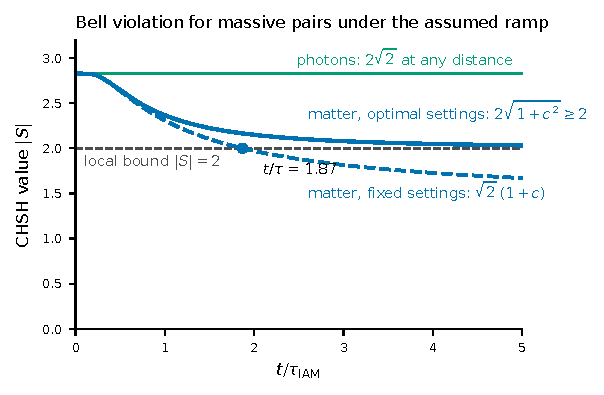
\includegraphics[width=0.62\textwidth]{figures/part4/fig_bell_decay.pdf}
\caption{CHSH value for entangled massive pairs under pointer-basis dephasing with the assumed ramp, coherence $c=1-E_q(t/\tau)/e$. With
settings re-optimised at each time the largest value is $2\sqrt{1+c^2}$, which never falls below the local bound; with the settings optimal for the
undecohered pair, $|S|=\sqrt2\,(1+c)$ crosses 2 at $c=0.414$, $t/\tau_{\rm IAM}=1.87$. Photon pairs stay at $2\sqrt2$. The ramp is assumed. \conjecture}
\end{figure}

IAM places nonlocal correlations in the photon sector, which in the dual-sector model carries no gravitational
decoherence and hence no duration (Chapter~\ref{ch:time}). A null geodesic has $d\tau=0$, so
two photons created together remain, in IAM's reading, at zero duration from each other
until one is absorbed. Correlations of any spatial separation then carry no signal and need
no propagation. \interp{} For entangled photons IAM predicts $|S|=2\sqrt2$ with no decay over any
distance. \prediction{} For entangled \emph{matter}, the gravitational channel of Chapter~\ref{ch:gravdec} dephases each body in its pointer basis and
multiplies the pair's coherence by $c(t)=1-D(t)$, with $D(t)=E_q(t/\tau_{\mathrm{IAM}})/e$ the assumed ramp of that chapter and
$\tau_{\mathrm{IAM}}$ from Eq.~\eqref{eq:tauIAM}. For pointer-basis dephasing the largest CHSH value is
\begin{equation}
 S_{\max}(t)=2\sqrt{1+c(t)^2}
\end{equation}
(Chapter~\ref{ch:entanglement}, Eq.~\eqref{eq:ent:smax}). \derived{} It stays above 2 for any remaining coherence and reaches 2 only when
the coherence is gone; with the settings that are optimal for the undecohered pair, $S=\sqrt2\,(1+c)$, which falls below 2 at $c<0.414$,
i.e.\ $D>0.586$. \calc{} The ramp itself is assumed. \conjecture
The CHSH values and the crossing time are derived in Appendix~\ref{app:der:quantum}.

\begin{checkbox}[title={Independent check: what entanglement distances show}]
Entanglement has been distributed over 1{,}200~km with photons~\cite{Yin2017} and between two
electron spins in NV centres 1.3~km apart~\cite{Hensen2015}, a ratio of about $10^3$. The
ratio is set by engineering, fibre and free-space losses, not by any matter-sector physics, so
entanglement distances do not test the sector split. \observed

The distinguishing prediction that remains is the one above. Entangled massive systems lose
Bell violation on the timescale $\tau_{\mathrm{IAM}}$ (with a sigmoidal onset if the assumed ramp
of Chapter~\ref{ch:gravdec} holds, an exponential one if the rate integral holds), while
entangled photons never do. \prediction{} For every massive system entangled to date (ions,
atoms, NV spins, superconducting circuits, silicon nanobeam oscillators~\cite{Riedinger2018} and
70~pg drumheads~\cite{Kotler2021}), $\tau_{\mathrm{IAM}}$ at physical densities is far
longer than the experiment. No test has yet been possible.
\end{checkbox}

\section{The exponent $5/2$}
Figure~\ref{fig:exponent_fit} shows the fitted activation coefficients against the exponent of the source term.
\begin{figure}[htbp]\centering
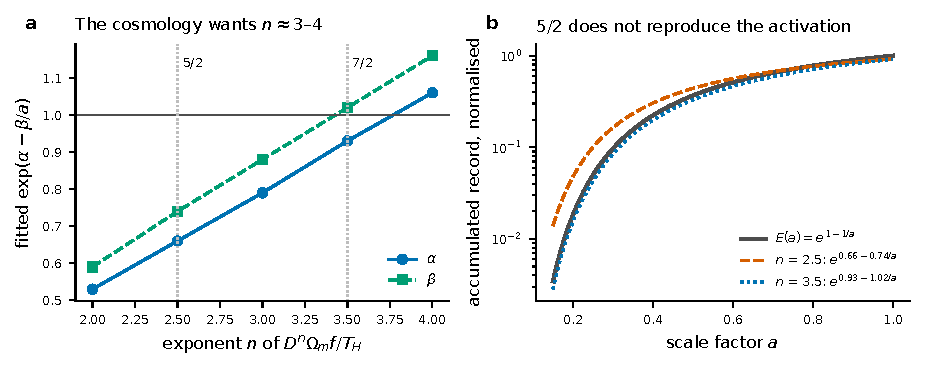
\includegraphics[width=\textwidth]{figures/part4/fig_exponent_fit.pdf}
\caption{(a) The coefficients of $\exp(\alpha-\beta/a)$ fitted to the accumulated record for the source terms $D^n\Omega_mf/T_H$ of Section~\ref{sec:numerics}: both pass 1 between $n=3$ and 4, bracketing 7/2. (b) The fitted forms for $n=5/2$ and $7/2$ against $E(a)=e^{1-1/a}$. \calc}\label{fig:exponent_fit}
\end{figure}

The exponent $5/2$ appears in the electron mass as $\alpha^{5/2}$. It does not carry over to the cosmic
information-production rate as $D(a)^{5/2}$. With the full $\Lambda$CDM background, the source term
$D^{5/2}\Omega_mf/T_H$ gives $E(a)\propto\exp(0.66-0.74/a)$, not the $\exp(1-1/a)$ the law uses; the two coefficients cross unity at
$n\approx3$--$4$, bracketing the analytic $n=7/2$ (Chapter~\ref{ch:theory}, Section~\ref{sec:numerics}). \calc{} The exponent $5/2$ therefore
appears in the electron mass of Chapter~\ref{ch:electronmass} and not in the cosmology, which takes $7/2$. Whether the
two exponents are related is open. \openprob

The split is clean: photon pairs keep the full Bell violation, and massive pairs are where the record enters. Anyone running entanglement with heavier and heavier objects is already aimed at the place where this is decided.
